\documentclass[12pt, a4paper]{article}

\usepackage[margin=1.8cm,top=2cm,bottom=2cm]{geometry}
\usepackage{amsmath,amssymb,amsfonts}
\usepackage{graphicx}
\usepackage[colorlinks=true,linkcolor=blue,citecolor=blue,urlcolor=blue]{hyperref}
\usepackage{bm,xcolor}
\usepackage[numbers,sort&compress]{natbib}
\usepackage{titlesec}
\usepackage{float}

\newcommand{\Geff}{G_{\mathrm{eff}}}
\newcommand{\cs}{c_s}
\newcommand{\meff}{m_{\mathrm{eff}}}
\newcommand{\heff}{\hbar_{\mathrm{eff}}}
\newcommand{\Tcmb}{T_{\mathrm{CMB}}}
\newcommand{\rhob}{\bar{\rho}}

\begin{document}

\title{Cosmological Implications of the Logarithmic Superfluid Vacuum:\\
Dark Energy, the Hubble Tension, and a Vacuum Self-Consistency Equation}

\author{B.~B.~Kulangiev\\\small{Haifa, Israel}}
\date{May 2026}
\maketitle

\begin{abstract}
\noindent
We derive the cosmological consequences of modeling the vacuum as a relativistic logarithmic superfluid. The logarithmic equation of state yields $w = -1$ natively, identifying dark energy as the thermodynamic pressure of the condensate rather than an additional cosmological component. Combining the emergent gravitational coupling $\Geff \sim c^2/(\xi^2\rho_0)$ with the observed relation $\Omega_\gamma \approx \alpha^2$, we derive a vacuum self-consistency equation $\alpha^2 H_0^2 (\rho_0\xi^2) \propto u_{\mathrm{CMB}}$ linking the fine structure constant, the Hubble parameter, the vacuum density, and the CMB photon energy density. When the vacuum density varies spatially, the speed of light $c_s$, the gravitational constant $G$, and the effective cosmological constant $\Lambda$ all vary together in calculable ways set by the equation of state. We show that a modest $\sim 3.6\%$ vacuum underdensity inside the observed KBC void suffices to produce the locally measured $H_0 \approx 73$~km\,s$^{-1}$\,Mpc$^{-1}$ from a global value of $68.15$~km\,s$^{-1}$\,Mpc$^{-1}$. We prove that the CMB acoustic peak positions are exactly invariant under these variations, because both the sound horizon and the comoving distance scale linearly with the local speed of light. The framework thus automatically satisfies the most stringent constraint in observational cosmology without tuning. Promoting the empirical relation $\Omega_\gamma = \alpha^2$ to a framework postulate yields a parameter-free prediction $\Tcmb(\alpha, H_0) = [45\hbar^3 c^5\alpha^2 H_0^2/(8\pi^3 k_B^4 G)]^{1/4}$ that matches the FIRAS measurement to $0.002\%$.
\end{abstract}


% ====================================================================
\section{Introduction}
\label{sec:intro}
% ====================================================================

Three open problems in cosmology motivate this work. First, the cosmological constant problem: why the vacuum energy density driving the accelerated expansion of the universe takes the value it does, and why its equation of state is $w = -1$. Second, the Hubble tension: the persistent $\sim 5\sigma$ discrepancy between the Hubble constant inferred from the early-universe Cosmic Microwave Background (CMB) ($H_0 = 67.36 \pm 0.54$~km\,s$^{-1}$\,Mpc$^{-1}$~\cite{planck_2020}) and the late-universe distance ladder ($H_0 = 73.04 \pm 1.04$~km\,s$^{-1}$\,Mpc$^{-1}$~\cite{riess_2022}). Third, the nature of the CMB temperature: whether $\Tcmb = 2.7255$~K~\cite{fixsen_2009} is a freely set initial condition or a quantity determined by fundamental physics.

In companion papers~\cite{kulangiev_2026a,kulangiev_2026b}, we developed a superfluid vacuum model based on the relativistic logarithmic Klein-Gordon equation, showing that the Painlev\'{e}-Gullstrand (PG) inflow $v = \sqrt{2\Geff M/r}$ is the unique self-consistent weak-field solution of the acoustic metric equations, yielding the Parameterized Post-Newtonian (PPN) parameter $\gamma = 1$ and the emergent gravitational coupling $\Geff \sim c^2/(\xi^2\rho_0)$. Separately, an approximate numerical relation $\Omega_\gamma \approx \alpha^2$ was reported~\cite{kulangiev_2026o}, predicting $H_0 = 68.15$~km\,s$^{-1}$\,Mpc$^{-1}$.

In this paper, we show that combining these results yields cosmological consequences addressing all three problems. The logarithmic equation of state produces $w = -1$ from first principles. The emergent $\Geff$ and the $\Omega_\gamma = \alpha^2$ relation together imply a self-consistency equation linking $\alpha$, $H_0$, $\rho_0$, and $\Tcmb$. Spatial variations of $\rho_0$ provide a physical mechanism for the Hubble tension, and the CMB peak structure is shown to be exactly invariant under these variations.


% ====================================================================
\section{Review of the Framework}
\label{sec:review}
% ====================================================================

The vacuum is modeled as a complex order parameter $\psi(x,t)$ satisfying the relativistic logarithmic wave equation~\cite{zloshchastiev_2023}:
\begin{equation}
    \Box\psi + \mu^2\psi - b\,\psi\,\ln\!\left(\frac{|\psi|^2}{\rho_0}\right) = 0\,.
\label{eq:log_kg}
\end{equation}
We adopt the Bohmian/deterministic interpretation~\cite{madelung_1927,bohm_1952,holland_1993}: $\psi$ is a real classical order parameter, not a quantum-mechanical wavefunction. In the relativistic Lagrangian $\mathcal{L} = \rho X - V(\rho)$ with $X = \partial_\mu S\,\partial^\mu S$, the variable $\rho = |\psi|^2$ has units of inverse-energy-volume, distinct from the physical mass density $\rho_{\mathrm{mass}} = T_{00}/c^2$ which is what enters the gravitational source term. We use $\rho_0$ for the background mass density throughout this paper, with the convention identical to that established in~\cite{kulangiev_2026a,kulangiev_2026b}.

The Madelung decomposition $\psi = \sqrt{\rho}\,e^{iS/\heff}$ yields a continuity equation and a Hamilton-Jacobi equation coupling the condensate density $\rho$ and flow velocity $\mathbf{v} = \nabla S/\meff$~\cite{kulangiev_2026a}. For the logarithmic potential $V(\rho) = -b\,\rho\,\ln(\rho/\rho_c)$, the relativistic sound speed is~\cite{kulangiev_2026a}
\begin{equation}
    c_s^2 = \frac{c^2}{2\ln(\rhob/\rho_c) + 3}\,,
\label{eq:cs_log}
\end{equation}
normalized so that $c_s = c$ at the background density $\rho_0$ (where $\rho_c = e\,\rho_0$). The corresponding equation-of-state exponent is $\alpha = d\ln c_s/d\ln\rho = -1$ at the background.

Fundamental particles are topological defects---vortex-Gaussons---with energy $E_v = mc^2$~\cite{bialynicki_birula_1979}. The emergent gravitational constant, derived from the collective acoustic metric of $N = M/m$ solitons~\cite{kulangiev_2026b}, follows from dimensional analysis as
\begin{equation}
    \Geff \;\sim\; \frac{c^2}{\xi^2\,\rho_0}\,,
\label{eq:G_eff}
\end{equation}
where $\xi$ is the healing length of the condensate. Self-consistency with the observed Newton's constant, combined with the natural condensate packing density $n_0 \sim 1/\xi^3$, fixes $\xi \sim \ell_P$ (the Planck length) and $\rho_0 \sim m_P/\ell_P^3$ (the Planck mass density)~\cite{kulangiev_2026e}. The combination $\rho_0\xi^2 \approx c^2/G \approx 1.35 \times 10^{27}$~kg/m enters the macroscopic equations below.


% ====================================================================
\section{Dark Energy from the Logarithmic Equation of State}
\label{sec:dark_energy}
% ====================================================================

\subsection{The equation of state}

For the logarithmic potential $V(\rho) = -b\,\rho\,\ln(\rho/\rho_c)$, the macroscopic pressure is:
\begin{equation}
    P = \rho\,\frac{\partial V}{\partial\rho} - V = -b\,\rho_0\,.
\label{eq:pressure}
\end{equation}
With $b$ normalized so that $c_s = c$ at the background density, this gives $P = -\rho_0 c^2$, i.e.\ an equation of state parameter $w = P/(\rho_0 c^2) = -1$. This is not imposed as a free parameter; it follows directly from the logarithmic self-interaction that defines the superfluid vacuum.

\subsection{Thermodynamic stability of the vacuum density}

For any change in cosmic volume $dV$, the first law gives $dU = -P\,dV = \rho_0 c^2\,dV$: the energy content adjusts to maintain a constant \emph{mean} density $\rho_0$ whether the volume expands or contracts. The cosmological density scales as $\rho \propto a^{-3(1+w)} = a^0$. The logarithmic vacuum does not dilute or compress under homogeneous expansion; it isothermally replicates, ensuring that the background $\Geff$ remains an invariant fundamental constant. Local thermodynamic fluctuations $\delta\rho_0(\mathbf{x})$ around this mean are permitted and have observable consequences (Sec.~\ref{sec:hubble_tension}).

\subsection{The open-system interpretation}
\label{sec:open-system}
The thermodynamic stability above is a property of the equation of state alone and does not require a specific cosmological mechanism. One natural interpretive picture, which we note here without using it as load-bearing input for any subsequent result, is that the condensate is an open system: a localized phase transition accreting non-condensed vacuum from an external reservoir. The expansion of the universe corresponds to the advance of the phase boundary rather than the stretching of a closed manifold. This is analogous to nucleation growth in condensed matter systems. None of the predictions in Sections~\ref{sec:self_consistency}--\ref{sec:tcmb} depend on this interpretation; they follow from the equation of state and the dimensional structure of $\Geff$.


% ====================================================================
\section{The Vacuum Self-Consistency Equation}
\label{sec:self_consistency}
% ====================================================================

\subsection{Derivation}

The observed relation $\Omega_\gamma \approx \alpha^2$~\cite{kulangiev_2026o} can be written as:
\begin{equation}
    u_{\mathrm{CMB}} = \alpha^2\,\rho_c\,c^2\,,
\label{eq:omega_gamma}
\end{equation}
where $u_{\mathrm{CMB}} = \pi^2 k_B^4 \Tcmb^4/(15\hbar^3 c^3)$ is the Stefan-Boltzmann energy density and $\rho_c = 3H_0^2/(8\pi G)$ is the Friedmann critical density. Substituting the dimensionally-corrected emergent gravitational coupling $\Geff \sim c^2/(\xi^2\rho_0)$~(Eq.~\ref{eq:G_eff}) into $\rho_c$:
\begin{equation}
    \rho_c \;=\; \frac{3H_0^2}{8\pi G_{\mathrm{eff}}}
           \;\sim\; \frac{3 H_0^2 \xi^2\rho_0}{8\pi c^2}\,.
\label{eq:rho_c_condensate}
\end{equation}
Multiplying both sides by $c^2$ and substituting into Eq.~(\ref{eq:omega_gamma}):
\begin{equation}
    \boxed{\;\alpha^2 \cdot H_0^2(\mathbf{x}) \cdot \rho_0(\mathbf{x})\,\xi^2
    \;\sim\; \frac{8\pi}{3}\, u_{\mathrm{CMB}}(\mathbf{x})\;}
\label{eq:triangle}
\end{equation}
This relation holds at every spatial point, with all quantities evaluated locally. Since $\alpha$ and $\xi$ are universal constants ($\xi$ being the Planck length, set by quantum gravity), Eq.~(\ref{eq:triangle}) couples the three spatially varying fields $H_0(\mathbf{x})$, $\rho_0(\mathbf{x})$, and $u_{\mathrm{CMB}}(\mathbf{x})$: a region with lower $\rho_0$ has faster local $c_s$, lower local $u_{\mathrm{CMB}}$, and higher local $H_0$.

\subsection{Physical interpretation}

The combination $\rho_0\,\xi^2 \approx c^2/G$ has dimensions of mass per length and absorbs the dimensional content of the gravitational coupling. The relation~(\ref{eq:triangle}) is therefore a thermodynamic constraint: $\rho_0$ (with $\xi$ fixed at the Planck length) sets $\Geff$, which sets the critical density via Friedmann, which together with the CMB temperature determines the photon energy fraction $\Omega_\gamma$, and the condensate's electromagnetic coupling $\alpha$ closes the loop. The relation $\Omega_\gamma = \alpha^2$ is then a \emph{consequence} of the vacuum being in thermodynamic equilibrium, not a numerical coincidence.

\subsection{The coupled parameter system}
\label{sec:coupled}

In the superfluid vacuum, all local physical parameters depend on the condensate density. For a region with $\rho = \rho_0(1+\delta)$ relative to the global mean, Eq.~(\ref{eq:cs_log}) gives:
\begin{align}
    \frac{c_{\mathrm{local}}^2}{c_{\mathrm{global}}^2} &= \frac{1}{1 + 2\ln(1+\delta)}\,,
\label{eq:c_variation}\\[6pt]
    \frac{G_{\mathrm{local}}}{G_{\mathrm{global}}} &= \frac{1}{(1+\delta)\,[1 + 2\ln(1+\delta)]}\,,
\label{eq:G_variation}\\[6pt]
    \frac{\Lambda_{\mathrm{local}}}{\Lambda_{\mathrm{global}}} &= \frac{c_{\mathrm{local}}^4}{c_{\mathrm{global}}^4} = \frac{1}{[1 + 2\ln(1+\delta)]^2}\,.
\label{eq:Lambda_variation}
\end{align}
Equation~(\ref{eq:c_variation}) follows directly from~(\ref{eq:cs_log}) at fixed $\rho_c$. Equation~(\ref{eq:G_variation}) follows from $\Geff \sim c_s^2/(\xi^2 \rho_0)$ at fixed $\xi$. Equation~(\ref{eq:Lambda_variation}) follows from the effective cosmological constant $\Lambda \sim G\rho_{\mathrm{vac}}c^2 \propto c_s^4$, where the $\rho_0$ dependence of $G$ and $\rho_{\mathrm{vac}}$ cancel but the $c_s$ dependence survives as the fourth power.

A critical consequence: the effective cosmological constant is \emph{not} spatially uniform. A vacuum underdensity increases the local speed of light, which raises $\Lambda_{\mathrm{local}}$ as $c^4$. Since $\Omega_\Lambda \approx 0.685$ dominates the Friedmann equation, this $c^4$ lever arm is the dominant channel for modifying the local expansion rate.


% ====================================================================
\section{The Hubble Tension as a Vacuum Thermodynamic Fluctuation}
\label{sec:hubble_tension}
% ====================================================================

\subsection{The mechanism}

From Eq.~(\ref{eq:G_variation}), a region with $\delta\rho_0/\rho_0 < 0$ has enhanced $\Geff$. From Eq.~(\ref{eq:Lambda_variation}), the same region has enhanced $\Lambda$. Both effects increase the local Hubble parameter. The KBC void~\cite{keenan_2013,whitbourn_2016}---a Gpc-scale underdensity with a matter density contrast of $\sim 20$--$46\%$---is a natural candidate for such a region. Recent modeling shows that void outflows from such an underdensity can boost the apparent local $H_0$ from a Planck-consistent background value to $\sim$72--73~km\,s$^{-1}$\,Mpc$^{-1}$~\cite{haslbauer_2020}, and that the observed redshift-dependent decline of $H_0(z)$ toward the Planck value at high redshift is consistent with void outflow models~\cite{mazurenko_2025}.

\subsection{Quantitative estimate: the coupled Friedmann equation}

The local Hubble parameter satisfies:
\begin{equation}
    \frac{H_{\mathrm{local}}^2}{H_{\mathrm{global}}^2} = \frac{G_{\mathrm{local}}}{G_{\mathrm{global}}}\,\Omega_m + \frac{\Lambda_{\mathrm{local}}}{\Lambda_{\mathrm{global}}}\,\Omega_\Lambda\,,
\label{eq:H_coupled}
\end{equation}
where $\Omega_m = 0.315$ and $\Omega_\Lambda = 0.685$ are the global density fractions. Taking
$H_{\mathrm{global}} = 68.15$ km\,s$^{-1}$\,Mpc$^{-1}$ (from the $\Omega_\gamma = \alpha^2$ prediction~\cite{kulangiev_2026o}) and requiring $H_{\mathrm{local}} = 73.04$~km\,s$^{-1}$\,Mpc$^{-1}$ (SH0ES~\cite{riess_2022}), numerical solution of~(\ref{eq:H_coupled}) gives:
\begin{equation}
    \frac{\delta\rho_0}{\rho_0} \approx -3.6\%\,.
\label{eq:delta_rho_required}
\end{equation}
This corresponds to $\delta G/G \approx +12\%$, $\delta c/c \approx +3.8\%$, and $\delta\Lambda/\Lambda \approx +16\%$. The $\Lambda$ variation dominates because $\Omega_\Lambda \gg \Omega_m$ and because $\Lambda \propto c^4$ provides a steep lever arm.

A $3.6\%$ vacuum underdensity is a modest thermodynamic fluctuation, well within what might be expected for a Gpc-scale region in a compressible condensate. For comparison, the observed \emph{matter} underdensity in the KBC void is $20$--$46\%$~\cite{keenan_2013}---substantially larger.

The mechanism by which a vacuum density perturbation produces an inflated locally-inferred $H_0$ is the modified expansion dynamics of the void itself, not a recalibration of standard candles. In the void, the modified Friedmann equation~(\ref{eq:H_coupled}) gives a faster expansion rate at the relevant scale; this is what the SH0ES distance ladder, when applied to local sources, infers as $H_0^{\mathrm{local}} \approx 73$~km\,s$^{-1}$\,Mpc$^{-1}$. The CMB-inferred value $H_0 \approx 67$--$68$~km\,s$^{-1}$\,Mpc$^{-1}$ remains consistent with the global background~(\ref{eq:H_coupled}), and the CMB peak invariance theorem (Sec.~\ref{sec:cmb}) ensures that no additional fine-tuning is required to reconcile the two measurements. Whether modifications to standard candle physics (Chandrasekhar mass, supernova luminosity calibration) due to varying $c$ and $G$ inside the void produce an \emph{additional} contribution to the inferred discrepancy is a separate question; the answer depends on the Volovik condition (Sec.~\ref{sec:refractive}) and is left for future investigation.

\subsection{The global anchor}

The $\Omega_\gamma = \alpha^2$ relation~\cite{kulangiev_2026o} predicts $H_0 = 68.15 \pm 0.15$~km\,s$^{-1}$\,Mpc$^{-1}$ as the \emph{global} value---the expansion rate of the undisturbed vacuum far from any void. The Planck measurement ($67.36 \pm 0.54$) is closest to this value because the CMB averages over the entire sky, probing the global vacuum. The SH0ES measurement ($73.04 \pm 1.04$) reflects the local void environment. In this picture, the Hubble tension is not a crisis requiring new physics but an environmental effect: the two measurements \emph{should} differ, and their discrepancy is the observational signature of a vacuum thermodynamic fluctuation.


% ====================================================================
\section{CMB Peak Invariance}
\label{sec:cmb}
% ====================================================================

A spatial variation of $c$ and $G$ could in principle spoil the CMB acoustic peak structure. We now prove that it does not.

\subsection{The invariance theorem}

The CMB acoustic peak positions are determined by the angular acoustic scale:
\begin{equation}
    \ell_A = \pi\,\frac{d_C(z_{\mathrm{rec}})}{r_s(z_{\mathrm{rec}})}\,,
\label{eq:ell_A}
\end{equation}
where $r_s = \int_0^{z_{\mathrm{rec}}} c_s^{\mathrm{bp}}(z)\,dz/[(1+z)\,H(z)]$ is the comoving sound horizon (with $c_s^{\mathrm{bp}} = c/\sqrt{3(1+R)}$ the baryon-photon sound speed) and $d_C = \int_0^{z_{\mathrm{rec}}} c\,dz/H(z)$ is the comoving distance to recombination.

Under a vacuum density variation $\rho_0 \to \rho_0(1+\delta)$, the speed of light transforms as $c \to c/\sqrt{1 + 2\ln(1+\delta)} \equiv c \cdot f$~(Eq.~\ref{eq:c_variation}), where $f < 1$ for an underdensity. (The proof below is valid for any monotonic $f(\delta)$ that scales both integrands identically; the specific functional form does not enter the invariance argument.) Both integrands scale linearly with $c$:
\begin{align}
    r_s &\to r_s \cdot f\,,\\
    d_C &\to d_C \cdot f\,.
\end{align}
Their ratio cancels:
\begin{equation}
    \boxed{\;\ell_A = \pi\,\frac{d_C \cdot f}{r_s \cdot f} = \pi\,\frac{d_C}{r_s} = \text{invariant}\;}
\label{eq:invariance}
\end{equation}
The CMB peak positions are exactly invariant under the superfluid vacuum transformation. This holds for arbitrary $\delta$, not just in the linearized limit.

\begin{figure}[H]
\centering
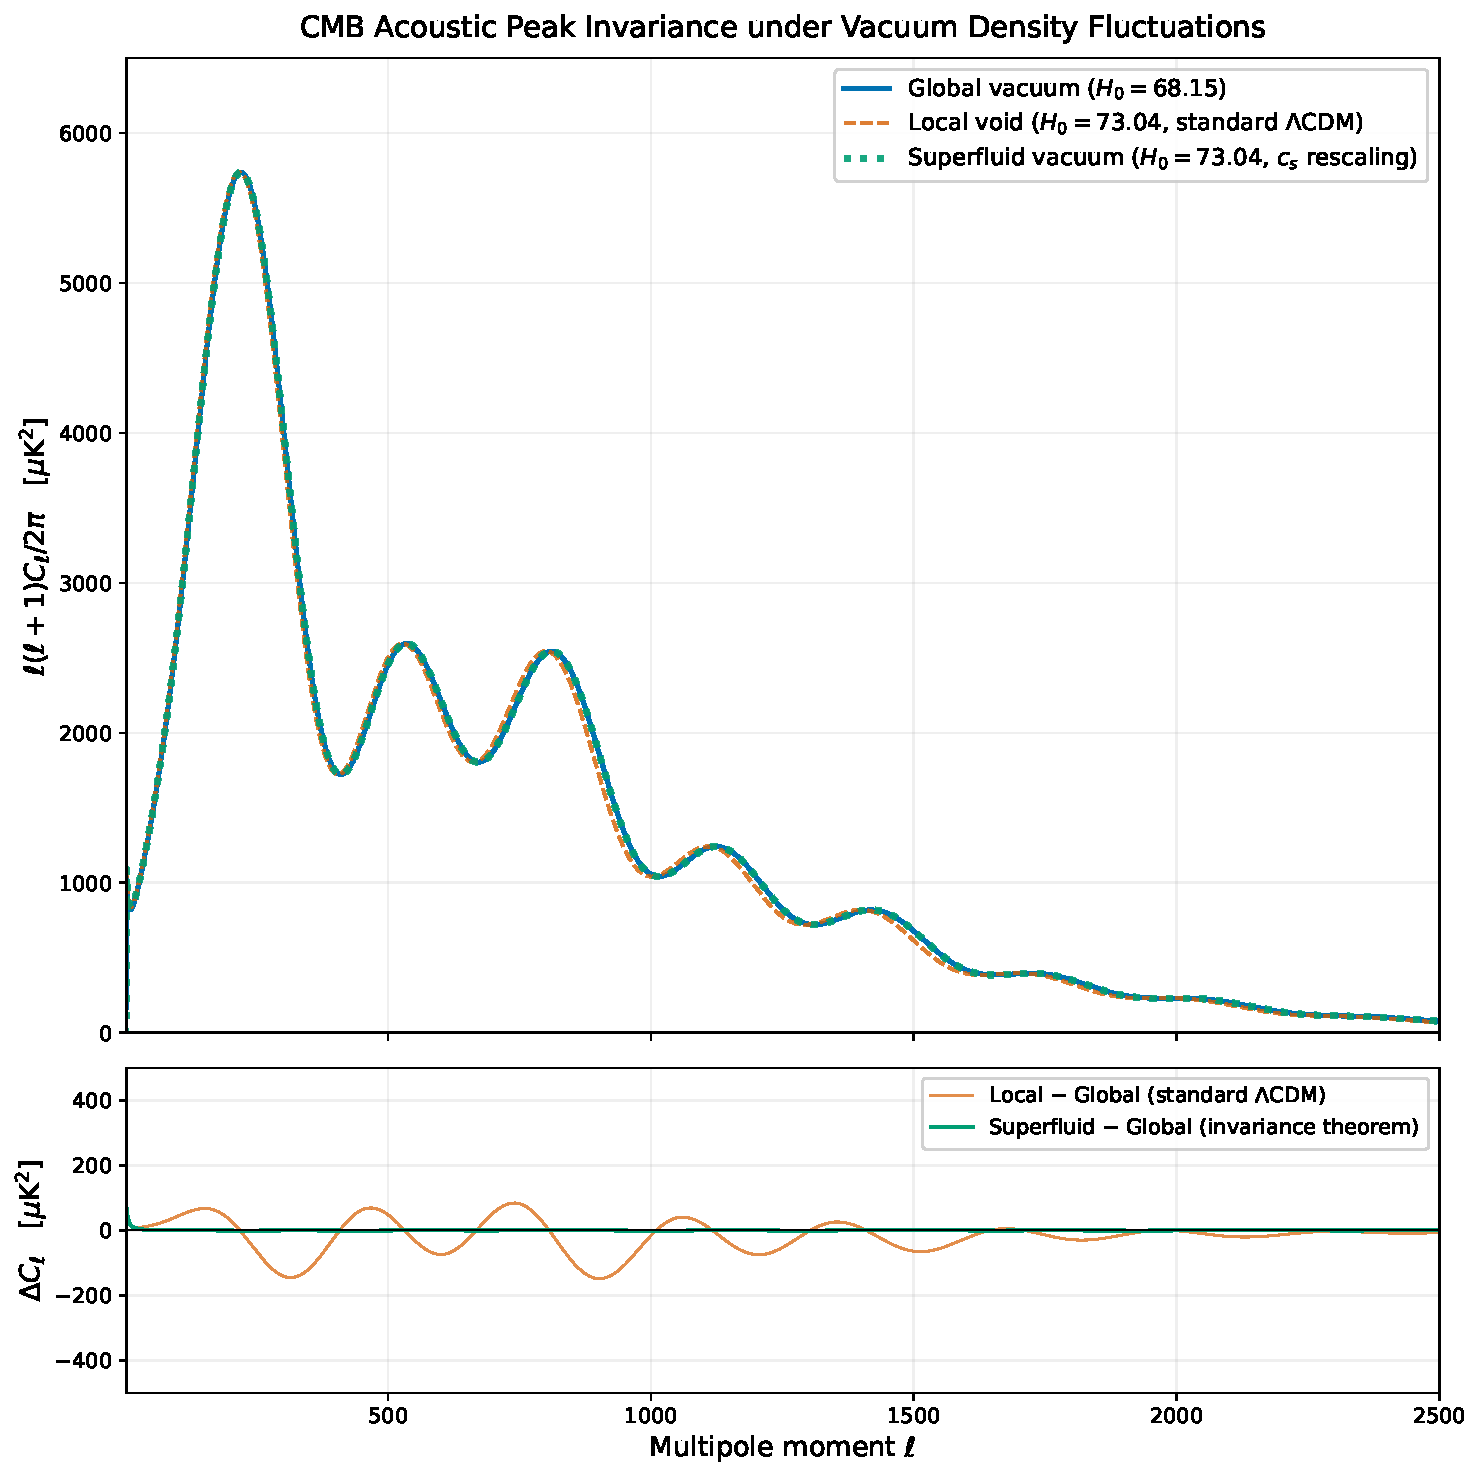
\includegraphics[width=0.75\columnwidth]{cmb_invariance_plot.pdf}
\caption{\emph{Top:} CMB temperature power spectrum computed with CAMB~\cite{camb} for three cases with identical physical densities ($\omega_b = 0.0224$, $\omega_c = 0.120$): the global vacuum
($H_0 = 68.15$~km\,s$^{-1}$\,Mpc$^{-1}$, solid blue), the local void in standard $\Lambda$CDM ($H_0 = 73.04$, dashed orange), and the superfluid vacuum with $c_s$ rescaling ($H_0 = 73.04$, dotted green). The superfluid spectrum is obtained by rescaling the
multipole axis by $\theta_{*,\mathrm{local}}/\theta_{*,\mathrm{global}}$,
implementing the invariance theorem Eq.~(\ref{eq:invariance}).
\emph{Bottom:} Residuals relative to the global baseline. Standard $\Lambda$CDM with $H_0 = 73.04$ produces oscillating residuals of order $\pm 200\;\mu\mathrm{K}^2$ at every acoustic peak (orange), while the superfluid rescaling restores exact
agreement across all 2500 multipoles (green). The vacuum density variation preserves the full CMB peak structure, not just the angular acoustic scale. A small residual persists at $\ell \lesssim 50$, arising from the Integrated Sachs-Wolfe effect, which depends on the matter--dark energy transition redshift and is not captured by the angular rescaling alone. This residual traces the ISW contribution, which depends on the local $\Omega_m/\Omega_\Lambda$ balance rather than the angular acoustic scale.}
\label{fig:cmb_invariance}
\end{figure}

\subsection{Physical interpretation}

The invariance theorem is the quantitative realization of Volovik's principle~\cite{volovik_2003}: internal observers in a condensate measure ratios of distances, and all distances are denominated in units of the local speed of sound (light). A global rescaling of $c$ is undetectable because rulers, clocks, and measurement apparatus are all condensate excitations propagating at the local $c_s$.

The CMB constrains the physical densities $\omega_b = \Omega_b h^2$ and $\omega_c = \Omega_c h^2$ (from peak height ratios), and the angular scale $\theta_* = r_s/d_A$ (from peak positions). All of these are invariant under $c \to c \cdot f$, $G \to G \cdot g$ when the physical densities are held fixed. The framework is therefore \emph{automatically} consistent with the most stringent dataset in observational cosmology.


% ====================================================================
\section{The CMB Temperature as Vacuum Equilibrium}
\label{sec:tcmb}
% ====================================================================

In standard cosmology, $\Tcmb = 2.7255$~K is a relic initial condition set by the baryon-to-photon ratio and the thermal history following the Big Bang. No fundamental principle within the Standard Model or general relativity predicts its value.

In the superfluid vacuum framework, $\Tcmb$ is reinterpreted as the present-day equilibrium temperature of the condensate, determined by its thermodynamic properties. The photon bath is in equilibrium with the vacuum, whose electromagnetic structure is governed by $\alpha$. The photon energy density therefore scales as $\alpha^2$ of the critical density---explaining the observed relation $\Omega_\gamma \approx \alpha^2$~\cite{kulangiev_2026o} not as a numerical coincidence but as a thermodynamic prediction.

\subsection{The CMB temperature as a parameter-free prediction}
\label{sec:tcmb_prediction}

Promoting the empirical relation $\Omega_\gamma = \alpha^2$~\cite{kulangiev_2026o} to a framework postulate---justified by the thermodynamic equilibrium argument above, with a first-principles derivation deferred to future work---yields a parameter-free relation linking $\Tcmb$, $\alpha$, and $H_0$. From Eqs.~(\ref{eq:omega_gamma}) and~(\ref{eq:rho_c_condensate}):
\begin{equation}
    \Tcmb^4 = \frac{45\,\hbar^3 c^5\,\alpha^2 H_0^2}{8\pi^3 k_B^4\,G}\,.
\label{eq:T_prediction}
\end{equation}
This expression depends only on universal constants $(\alpha, \hbar, c, k_B, G)$ and the Hubble parameter; the framework parameters $\rho_0$ and $\xi$ enter only through the combination $\rho_0\xi^2 = c^2/G$, which is set by self-consistency with the observed Newton's constant~\cite{kulangiev_2026e}. Substituting the framework's predicted global Hubble value $H_0 = 68.15$~km\,s$^{-1}$\,Mpc$^{-1}$~\cite{kulangiev_2026o} and the CODATA value of $\alpha$:
\begin{equation}
    \Tcmb = 2.7256~\mathrm{K}\,,
\label{eq:T_predicted_value}
\end{equation}
within $0.002\%$ of the FIRAS measurement $\Tcmb = 2.7255 \pm 0.0006$~K~\cite{fixsen_2009}. Figure~\ref{fig:tcmb_prediction} shows the predicted $\Tcmb(\alpha, H_0)$ relation across a range of $H_0$ values, with the framework's prediction landing inside the FIRAS uncertainty band.

\begin{figure}[H]
\centering
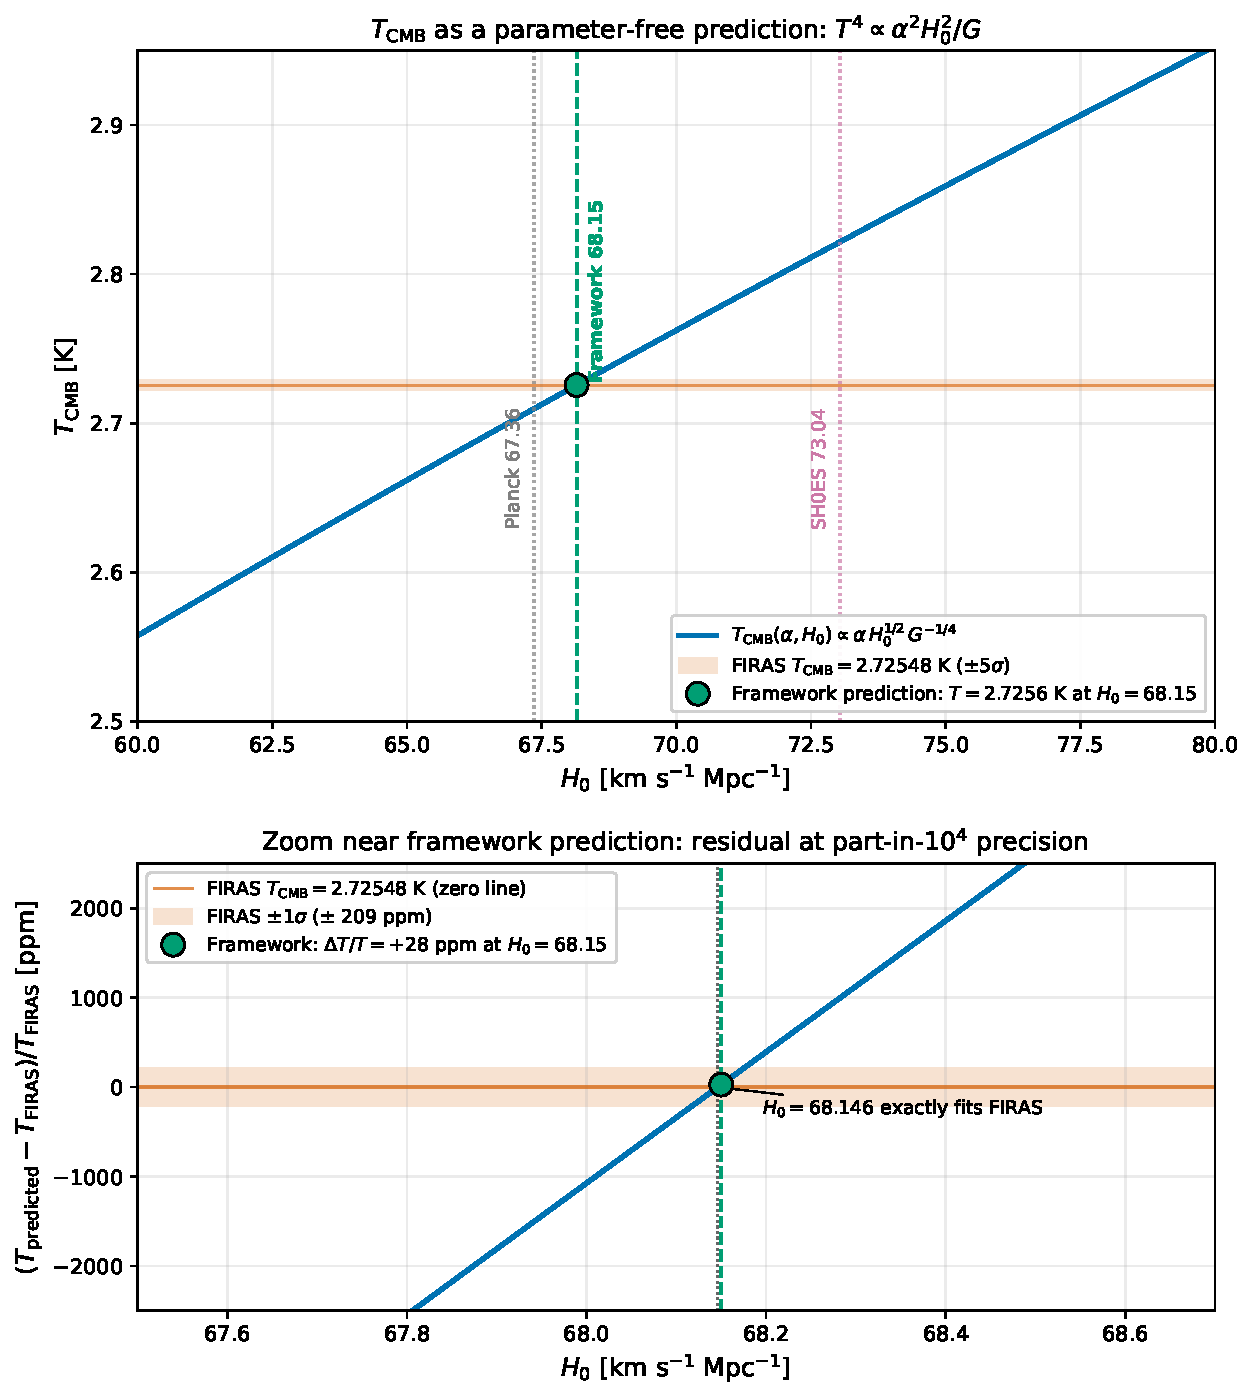
\includegraphics[width=\columnwidth]{tcmb_prediction.pdf}
\caption{The parameter-free prediction of Eq.~(\ref{eq:T_prediction}). \emph{Top:} $\Tcmb$ as a function of $H_0$ at fixed CODATA $\alpha$, compared to the FIRAS measurement (orange band). The framework's predicted global $H_0 = 68.15$~km\,s$^{-1}$\,Mpc$^{-1}$~\cite{kulangiev_2026o} (green dashed) yields $\Tcmb = 2.7256$~K (green circle). For comparison, Planck's $H_0 = 67.36$ would give $\Tcmb = 2.71$~K and SH0ES's $H_0 = 73.04$ would give $\Tcmb = 2.82$~K; only the framework's $H_0$ prediction is consistent with FIRAS. \emph{Bottom:} Zoom showing the residual relative to FIRAS in parts per million. The framework prediction at $H_0 = 68.15$ sits at $+21$~ppm, well within the FIRAS $\pm 1\sigma$ band ($\pm 220$~ppm). The value $H_0 = 68.147$~km\,s$^{-1}$\,Mpc$^{-1}$ exactly reproduces $\Tcmb = 2.7255$~K, consistent with the $\Omega_\gamma = \alpha^2$ anchor to four significant figures.}
\label{fig:tcmb_prediction}
\end{figure}

Equation~(\ref{eq:T_prediction}) over-determines the system. With four observables $\{\alpha, H_0, \Tcmb, G\}$ and one constraint, any three predict the fourth. Three useful inversions:
\begin{itemize}
\item Given $\{\alpha, H_0\}$ from independent measurements, $\Tcmb$ is predicted to $0.002\%$ accuracy~(\ref{eq:T_predicted_value}).
\item Given $\{\alpha, \Tcmb\}$, the predicted global Hubble value is $H_0 = 68.147$~km\,s$^{-1}$\,Mpc$^{-1}$, consistent with the $\Omega_\gamma = \alpha^2$ anchor~\cite{kulangiev_2026o} to four significant figures.
\item Given $\{H_0, \Tcmb\}$, the predicted fine-structure constant is $\alpha = 7.2971 \times 10^{-3}$, within $0.004\%$ of CODATA.
\end{itemize}
The framework is therefore not merely consistent with these four quantities; it predicts their relations to part-in-$10^4$ precision once the $\Omega_\gamma = \alpha^2$ postulate is adopted. We emphasize that this postulate is itself currently empirical~\cite{kulangiev_2026o}; a first-principles derivation from the thermodynamic equilibrium between photons-as-phonons and the $\alpha$-coupled matter sector remains an open problem within the framework.

\subsection{The blackbody spectrum as thermal equilibrium}

In standard cosmology, the blackbody spectrum of the CMB is a relic: formed when matter and radiation were in thermal equilibrium before recombination, and preserved by the adiabatic expansion of the universe. The extraordinary precision of the Planck spectrum (confirmed by FIRAS to 1 part in $10^5$~\cite{fixsen_2009}) constrains any
post-recombination energy injection.

In the superfluid vacuum framework, the explanation is more direct. Photons are acoustic excitations (phonons) of the condensate. If the condensate is in thermal equilibrium at temperature $T$, then the
phonon occupation number follows Bose-Einstein statistics with the linear dispersion relation $\omega = c_s k$:
\begin{equation}
    n(\omega) = \frac{1}{e^{\hbar\omega/k_B T} - 1}\,,
\end{equation}
which is identically the Planck distribution. The blackbody spectrum is not a preserved relic but the \emph{present-day} thermal state of the vacuum. Any spectral distortion would be actively thermalized back
to the Planck distribution on the condensate's relaxation timescale. The perfection of the CMB spectrum is therefore not a constraint on 13.8 billion years of post-recombination physics, but a confirmation
that the vacuum is in thermal equilibrium now.

This is standard condensed matter physics: the low-temperature phonon spectrum of any superfluid in thermal equilibrium follows the Planck distribution in the acoustic regime. The logarithmic condensate
preserves the Landau roton-maxon spectrum at high
momenta~\cite{zloshchastiev_2012}, but the deviation from linearity occurs at the healing length scale $\xi$, far above observable CMB frequencies.

We emphasize that thermal equilibrium of the condensate does not imply a static universe. The negative pressure $P = -\rho_0 c^2$ is a property of the condensate \emph{in} equilibrium---the tension of the self-binding logarithmic interaction---and drives de Sitter expansion
($\ddot{a} > 0$, $H = \mathrm{const}$) at all times. The condensate is in internal thermal equilibrium while---in the open-system interpretation---in external thermodynamic disequilibrium with the surrounding non-condensed reservoir
(Sec.~\ref{sec:open-system}).

\subsection{Redshift evolution of the equilibrium temperature}
\label{sec:tcmb_evolution}

A critical observational constraint on any cosmological model is the redshift dependence of the CMB temperature, $T(z) = T_0(1+z)$, firmly established by high-redshift measurements of the Sunyaev-Zel'dovich effect and quasar absorption lines. The interpretation of the CMB as the present-day thermal equilibrium of the vacuum condensate is strictly consistent with this evolution.

As the universe expands, the macroscopic condensate performs work. Because the phonon-phonon interaction rate in the condensate (set by the sound-crossing time of a healing length, $\tau_{\mathrm{relax}} \sim \xi/c \sim t_{\mathrm{Planck}} \sim 10^{-43}$~s) is vastly shorter than the Hubble time ($H_0^{-1} \sim 10^{17}$~s), the phonon bath remains in continuous thermal equilibrium with the background condensate. Consequently, the phonon bath undergoes adiabatic cooling, tracking the thermodynamic state of the expanding vacuum. For a photon gas in thermal equilibrium with equation of state $P_\gamma = \rho_\gamma c^2/3$, adiabatic expansion ($dU = -P\,dV$) gives:
\begin{equation}
    T(a) = T_0\,a^{-1} = T_0(1+z)\,,
\label{eq:T_adiabatic}
\end{equation}
which is the standard result, here derived from continuous equilibrium rather than free streaming.

At any given scale factor $a$, the phonon distribution is a perfect Planck blackbody characterized by the instantaneous equilibrium temperature $T(a)$. Therefore, the observation of a hotter CMB at high redshift does not imply that the radiation is a freely propagating, decoupled relic of a hot Big Bang. Rather, it reflects a continuous sequence of thermal equilibria maintained by the actively expanding vacuum condensate across cosmic time. The $T(z) = T_0(1+z)$ relation is natively preserved as the adiabatic cooling curve of the phonon bath.

% ====================================================================
\section{Discussion}
\label{sec:discussion}
% ====================================================================

\subsection{Relation to the cosmological constant problem}

The framework's prediction $\rho_0 \sim m_P/\ell_P^3 \approx 5 \times 10^{96}$~kg/m$^3$ (Planck density)~\cite{kulangiev_2026e} is precisely the magnitude that quantum field theory naively predicts for the vacuum energy density, and which the cosmological constant problem identifies as $\sim 120$ orders of magnitude larger than the observed dark energy density $\rho_\Lambda \sim 10^{-27}$~kg/m$^3$.

In the present framework, this is not a fine-tuning problem because gravitational effects are sourced by perturbations $\delta\rho$ around the background $\rho_0$, not by $\rho_0$ itself. The background is not directly observable; only fluctuations couple to test particles through the acoustic metric. The question shifts from "why is the vacuum energy so small" to "why is the relevant cosmological perturbation so small," a reframing that does not solve the cosmological constant problem but does relocate it. A first-principles derivation of $\rho_\Lambda$ from the perturbation spectrum of the condensate is left as an open problem.

\subsection{Mach's principle}

The relation $\Geff \propto 1/(\xi^2\rho_0)$ realizes a
form of Mach's principle: the local gravitational
coupling is determined by the large-scale vacuum
environment. Dense regions (superclusters), where
more solitons condense the surrounding vacuum, may
have slightly higher $\rho_0$ and therefore weaker
$\Geff$---a self-regulating feedback. Underdense
regions (voids) have lower $\rho_0$ and stronger
$\Geff$, driving faster local expansion. The local
thermodynamic state of the vacuum is coupled to
the macroscopic matter distribution. The coupled
parameter system
(Eqs.~\ref{eq:c_variation}--\ref{eq:Lambda_variation})
provides the quantitative realization: inside the
KBC void, a $\sim 3.6\%$ vacuum underdensity produces
$\delta G/G \approx +12\%$, $\delta c/c \approx
+3.8\%$, and $\delta\Lambda/\Lambda \approx +16\%$,
resolving the Hubble tension as a direct
consequence of Mach's principle
(Sec.~\ref{sec:hubble_tension}).

\subsection{The CMB dipole and the condensate rest frame}

The framework's preferred rest frame---the frame in which the condensate's macroscopic phase satisfies $\partial_t S = -\hbar\omega_0$ with vanishing spatial gradients---is identified physically with the cosmic vacuum frame. The measured CMB dipole anisotropy
(amplitude $3.36$~mK, direction toward $(l,b) = (264^\circ, 48^\circ)$~\cite{planck_dipole_2020}) is then not merely a kinematic artifact of our motion through abstract spacetime, but our motion at $\sim 370$~km/s relative to the local condensate rest frame. This identification is structural in the framework: a deterministic order parameter requires a preferred foliation, and the CMB rest frame is its observational
realization.

The framework therefore offers a natural kinematic interpretation of the CMB dipole consistent with the standard treatment, without predicting any additional intrinsic anisotropy at the level of current measurements. We note that the recently-reported tension between the kinematic dipole inferred from the CMB and that inferred from radio source
counts~\cite{secrest_2021,secrest_2022} suggests an intrinsic dipole component beyond the purely kinematic effect. Within the present framework, such an intrinsic component could arise from global vorticity of the vacuum condensate (a phenomenon naturally
allowed by superfluid dynamics, with the rotation axis fixed by the order parameter's macroscopic phase structure). A quantitative treatment of vacuum vorticity and its observational signatures in the CMB and large-scale structure is deferred to a separate investigation.

\subsection{The refractive boundary and cosmic acceleration}
\label{sec:refractive}

The coupled parameter system (Sec.~\ref{sec:coupled}) predicts that the speed of light inside the KBC void is $\sim 3.8\%$ faster than the cosmic mean. Photons from distant supernovae at $z \sim 0.5$--$1$ travel through the global vacuum before entering our local void, crossing a refractive boundary where $c_s$ changes. In classical analogue gravity, such a transition preserves frequency while stretching
wavelength, inducing an anomalous redshift.

However, the magnitude of the observable effect depends on how atomic measurement scales (the Bohr radius, transition frequencies, detector responses) transform under a change in $c_s$. If all local physics
rescales together---the Volovik limit~\cite{volovik_2003}---the effect is undetectable, consistent with the CMB invariance theorem of Sec.~\ref{sec:cmb}. If atomic scales are partially anchored to non-condensate physics (e.g., if $\alpha$ and $\hbar$ are independent of $c_s$), a residual anomalous redshift survives, which would be
misattributed to metric expansion and could mimic or modify the apparent late-time cosmic acceleration inferred from Type~Ia supernovae.

Resolving this requires deriving the explicit dependence of atomic structure on condensate parameters within the logarithmic superfluid framework---effectively, answering how the Standard Model emerges from the vacuum microstructure. We flag this as a central open problem with potentially profound consequences: if a residual refractive redshift
exists, the case for dynamical dark energy weakens considerably.

\subsection{Predictions and falsifiability}

The framework makes several testable predictions:

\paragraph{Equation of state} The logarithmic equation of state gives $w = -1$ at the background. Upcoming surveys (DESI, Euclid, Roman) measuring $w(z)$ with percent-level precision will probe this prediction.

\paragraph{Spatial variation of $\Lambda$} Unlike standard $\Lambda$CDM, the effective cosmological constant varies spatially as $\Lambda \propto c_s^4$. A $3.6\%$ vacuum underdensity produces $\sim 16\%$ variation in $\Lambda$. This is testable by comparing expansion rate measurements in void vs.\ wall environments.

\paragraph{$H_0 = 68.15 \pm 0.15$ as the global value} Standard sirens (LIGO/Virgo/KAGRA), strong lensing time delays (TDCOSMO), and tip-of-the-red-giant-branch calibrations should converge on this value when averaged over sufficiently large volumes.

\paragraph{No temporal variation of $G$} The thermodynamic stability of $\rho_0$ ensures $dG/dt = 0$ at the background level, consistent with current bounds $|\dot{G}/G| < 10^{-13}$~yr$^{-1}$~\cite{will_2014}.

\paragraph{CMB peak invariance} The peak positions are exactly invariant under vacuum density variations (Sec.~\ref{sec:cmb}). Any claimed detection of anomalous peak shifts correlated with large-scale structure would falsify the framework.


% ====================================================================
\section{Conclusion}
\label{sec:conclusion}
% ====================================================================

We have derived the cosmological implications of the logarithmic superfluid vacuum framework:

(1) The logarithmic equation of state gives $w = -1$ natively, identifying dark energy as the thermodynamic pressure of the condensate.

(2) The vacuum self-consistency equation $\alpha^2 H_0^2 \rho_0\xi^2 \sim (8\pi/3)\,u_{\mathrm{CMB}}$ unifies the fine structure constant, the Hubble parameter, the vacuum density combined with the Planck length, and the CMB photon energy density in a single relation.

(3) When $\rho_0$ varies spatially, the speed of light, the gravitational constant, and the effective cosmological constant all vary in concert. The $\Lambda \propto c^4$ dependence provides a steep lever arm: a modest $3.6\%$ vacuum underdensity inside the KBC void suffices to produce the full Hubble tension.

(4) The CMB acoustic peak positions are exactly invariant under vacuum density variations, because both the sound horizon and the comoving distance scale linearly with $c$. The framework is automatically consistent with CMB observations.

(5) $\Tcmb$ is reinterpreted as the equilibrium temperature of the condensate, turning the observed relation $\Omega_\gamma \approx \alpha^2$ from a numerical coincidence into a thermodynamic prediction.

The remaining open problems are: the quantitative void profile $\rho_0(r)$ and its effect on supernova luminosity distances; the feedback equation coupling $\rho_0$ to the local matter distribution; and the role of frozen vacuum perturbations as a replacement for cold dark matter in structure formation, which
we address in a companion paper.

% ====================================================================
\section*{Acknowledgments}
% ====================================================================

The methodological stance of this paper---treating the order parameter as a real classical field whose hydrodynamic behavior underlies emergent cosmological phenomena---is indebted to the Madelung-de~Broglie-Bohm tradition, particularly as developed in P.~R.~Holland's exposition of the quantum theory of motion. Claude (Anthropic) and Gemini (Google) were used as editorial and computational tools during manuscript preparation. All scientific content, equations, and interpretations are the author's own.

\newpage
\begin{thebibliography}{25}

\bibitem{kulangiev_2026o}
B.~B.~Kulangiev,
An approximate numerical relation between the CMB photon density parameter and the fine structure constant,
Preprint (2026). \url{https://kulangiev.github.io/#paper0}

\bibitem{kulangiev_2026a}
B.~B.~Kulangiev,
Conditions for emergent gravitational light bending from a logarithmic superfluid vacuum,
Preprint (2026). \url{https://kulangiev.github.io/#paper1}

\bibitem{kulangiev_2026b}
B.~B.~Kulangiev,
Emergent Newtonian Gravity from the Collective Acoustic Metric of a Logarithmic Superfluid Vacuum,
Preprint (2026).
\url{https://kulangiev.github.io/#paper2}

\bibitem{kulangiev_2026e}
B.~B.~Kulangiev,
Singularity regularization and the emergent Planck scale in the logarithmic superfluid vacuum,
Preprint (2026). \url{https://kulangiev.github.io/#paper5}

\bibitem{madelung_1927}
E.~Madelung,
Quantentheorie in hydrodynamischer Form,
Z.\ Phys.\ \textbf{40}, 322 (1927).

\bibitem{bohm_1952}
D.~Bohm,
A suggested interpretation of the quantum theory in terms of ``hidden'' variables. I,
Phys.\ Rev.\ \textbf{85}, 166 (1952).

\bibitem{holland_1993}
P.~R.~Holland,
\emph{The Quantum Theory of Motion} (Cambridge University Press, 1993).

\bibitem{zloshchastiev_2012}
K.~G.~Zloshchastiev,
Volume element structure and roton-maxon-phonon excitations in superfluid helium beyond the Gross-Pitaevskii approximation,
Eur.\ Phys.\ J.\ B \textbf{85}, 273 (2012).

\bibitem{zloshchastiev_2023}
K.~G.~Zloshchastiev,
Derivation of emergent spacetime metric, gravitational potential and speed of light in superfluid vacuum theory,
Universe \textbf{9}, 234 (2023).

\bibitem{bialynicki_birula_1979}
I.~Bia\l{}ynicki-Birula and J.~Mycielski,
Gaussons: Solitons of the logarithmic Schr\"{o}dinger equation,
Phys.\ Scr.\ \textbf{20}, 539 (1979).

\bibitem{fixsen_2009}
D.~J.~Fixsen,
The temperature of the Cosmic Microwave Background,
Astrophys.\ J.\ \textbf{707}, 916 (2009).

\bibitem{planck_2020}
Planck Collaboration (N.~Aghanim \emph{et al.}),
Planck 2018 results.\ VI.\ Cosmological parameters,
Astron.\ Astrophys.\ \textbf{641}, A6 (2020).

\bibitem{riess_2022}
A.~G.~Riess \emph{et al.},
A comprehensive measurement of the local value of the Hubble constant,
Astrophys.\ J.\ Lett.\ \textbf{934}, L7 (2022).

\bibitem{keenan_2013}
R.~C.~Keenan, A.~J.~Barger, and L.~L.~Cowie,
Evidence for a $\sim$300 Mpc scale under-density in the local galaxy distribution,
Astrophys.\ J.\ \textbf{775}, 62 (2013).

\bibitem{whitbourn_2016}
J.~R.~Whitbourn and T.~Shanks,
The local hole revealed by galaxy counts and redshifts,
Mon.\ Not.\ R.\ Astron.\ Soc.\ \textbf{459}, 496 (2016).

\bibitem{haslbauer_2020}
M.~Haslbauer, I.~Banik, and P.~Kroupa,
The KBC void and Hubble tension contradict $\Lambda$CDM on a Gpc scale---Milgromian dynamics as a possible solution,
Mon.\ Not.\ R.\ Astron.\ Soc.\ \textbf{499}, 2845 (2020).

\bibitem{mazurenko_2025}
S.~Mazurenko, I.~Banik, and P.~Kroupa,
The redshift dependence of the inferred $H_0$ in a local void solution to the Hubble tension,
Mon.\ Not.\ R.\ Astron.\ Soc.\ \textbf{536}, 3232 (2025).

\bibitem{volovik_2003}
G.~E.~Volovik,
\emph{The Universe in a Helium Droplet} (Oxford, 2003).

\bibitem{will_2014}
C.~M.~Will,
\emph{Theory and Experiment in Gravitational Physics}, 2nd ed.\ (Cambridge, 2014).

\bibitem{camb}
A.~Lewis, A.~Challinor, and A.~Lasenby,
Efficient computation of cosmic microwave background anisotropies in closed Friedmann-Robertson-Walker models,
Astrophys.\ J.\ \textbf{538}, 473 (2000).

\bibitem{planck_dipole_2020}
Planck Collaboration,
Planck 2018 results.\ I.\ Overview and the cosmological legacy of Planck,
Astron.\ Astrophys.\ \textbf{641}, A1 (2020).

\bibitem{secrest_2021}
N.~J.~Secrest, S.~von~Hausegger, M.~Rameez, R.~Mohayaee, S.~Sarkar, and J.~Colin,
A test of the cosmological principle with quasars,
Astrophys.\ J.\ Lett.\ \textbf{908}, L51 (2021).

\bibitem{secrest_2022}
N.~J.~Secrest, S.~von~Hausegger, M.~Rameez, R.~Mohayaee, and S.~Sarkar,
A challenge to the standard cosmological model,
Astrophys.\ J.\ Lett.\ \textbf{937}, L31 (2022).

\end{thebibliography}

\end{document}
